%% : Introduction à l'effet Marangoni

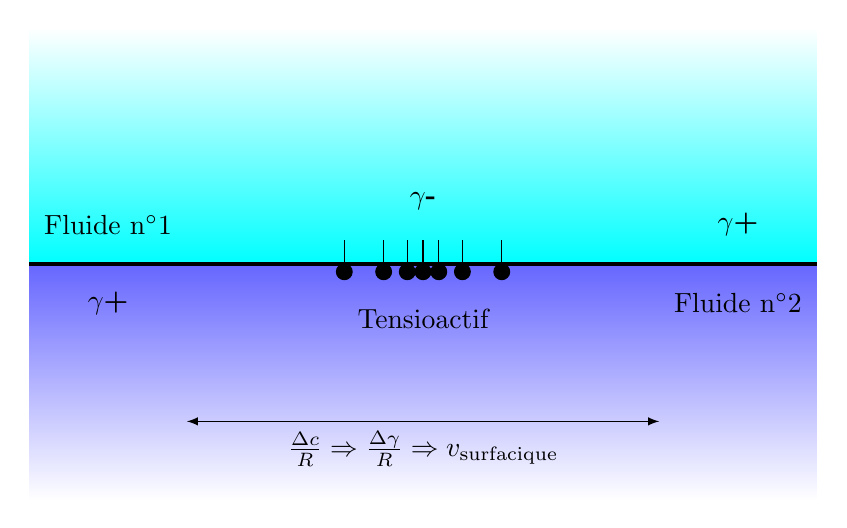
\begin{tikzpicture}[scale=1]
  \shade [top color = white, bottom color=cyan] (-5,0) -- (5,0) -- (5,3) -- (-5,3) -- cycle;
  \shade [top color = blue!60, bottom color = white] (-5,0) -- (5,0) -- (5,-3) -- (-5,-3) -- cycle;
  \draw[very thick] (-5,0) -- (5,0);

  \draw (-4,.5) node{Fluide n$^{\circ}1$};
  \draw (4,-.5) node{Fluide n$^{\circ}2$};
  \draw (4,.5) node{$\boldsymbol{\gamma}\textbf{+}$};
  \draw (-4,-.5) node{$\boldsymbol{\gamma}\textbf{+}$};
  \foreach \x in {-1,-.5,-.2, 0, .2, .5, 1} \draw[fill=black] (\x,-.1) circle (.1);
  
           %\foreach \x in {1,2,3} {$x=\x$, }
  \foreach \x in {-1,-.5,-.2,0,.2,.5,1} \draw[black] (\x,0)--(\x,.3) ;
  
  \draw (0,.8) node{$\boldsymbol{\gamma}\textbf{-}$};
  \draw (0,-.7) node{Tensioactif};
  
  \draw [latex-latex](-3,-2)--(3,-2) node[below, midway]{ $\frac{\Delta c}{R} \Rightarrow \frac{\Delta \gamma}{R} \Rightarrow v_{\rm surfacique}$};
 
\end{tikzpicture}
